
\documentclass[letterpaper,hide notes,xcolor={table,svgnames},pdftex,10pt]{beamer}
\def\showexamples{t}


%\usepackage[svgnames]{xcolor}

%% Demo talk
%\documentclass[letterpaper,notes=show]{beamer}

\usecolortheme{crane}
\setbeamertemplate{navigation symbols}{}

\usetheme{MyPittsburgh}
%\usetheme{Frankfurt}

%\usepackage{tipa}

\usepackage{hyperref}
\usepackage{graphicx,xspace}
\usepackage[normalem]{ulem}
\usepackage{multicol}

\newcommand\SF[1]{$\bigstar$\footnote{SF: #1}}

\usepackage[default]{sourcesanspro}
\usepackage[T1]{fontenc}

\newcounter{tmpnumSlide}
\newcounter{tmpnumNote}

% old question code
%\newcommand\question[1]{{$\bigstar$ \small \onlySlide{2}{#1}}}
% \newcommand\nquestion[1]{\ifdefined \presentationonly \textcircled{?} \fi \note{\par{\Large \textbf{?}} #1}}
% \newcommand\nanswer[1]{\note{\par{\Large \textbf{A}} #1}}


 \newcommand\mnote[1]{%
   \addtocounter{tmpnumSlide}{1}
   \ifdefined\showcues {~\tiny\fbox{\arabic{tmpnumSlide}}}\fi
   \note{\setlength{\parskip}{1ex}\addtocounter{tmpnumNote}{1}\textbf{\Large \arabic{tmpnumNote}:} {#1\par}}}

\newcommand\mmnote[1]{\note{\setlength{\parskip}{1ex}#1\par}}

%\newcommand\mnote[2][]{\ifdefined\handoutwithnotes {~\tiny\fbox{#1}}\fi
% \note{\setlength{\parskip}{1ex}\textbf{\Large #1:} #2\par}}

%\newcommand\mnote[2][]{{\tiny\fbox{#1}} \note{\setlength{\parskip}{1ex}\textbf{\Large #1:} #2\par}}

\newcommand\mquestion[2]{{~\color{red}\fbox{?}}\note{\setlength{\parskip}{1ex}\par{\Large \textbf{?}} #1} \note{\setlength{\parskip}{1ex}\par{\Large \textbf{A}} #2\par}\ifdefined \presentationonly \pause \fi}

\newcommand\blackboard[1]{%
\ifdefined   \showblackboard
  {#1}
  \else {\begin{center} \fbox{\colorbox{blue!30}{%
         \begin{minipage}{.95\linewidth}%
           \hspace{\stretch{1}} Some space intentionally left blank; done at the blackboard.%
         \end{minipage}}}\end{center}}%
         \fi%
}



%\newcommand\q{\tikz \node[thick,color=black,shape=circle]{?};}
%\newcommand\q{\ifdefined \presentationonly \textcircled{?} \fi}

\usepackage{listings}
\lstset{%
  keywordstyle=\bfseries,
  aboveskip=15pt,
  belowskip=15pt,
  captionpos=b,
  identifierstyle=\ttfamily,
  escapeinside={(*@}{@*)},
  stringstyle=\ttfamiliy,
  frame=lines,
  numbers=left, basicstyle=\scriptsize, numberstyle=\tiny, stepnumber=0, numbersep=2pt}

\usepackage{siunitx}
\newcommand\sius[1]{\num[group-separator = {,}]{#1}\si{\micro\second}}
\newcommand\sims[1]{\num[group-separator = {,}]{#1}\si{\milli\second}}
\newcommand\sins[1]{\num[group-separator = {,}]{#1}\si{\nano\second}}
\sisetup{group-separator = {,}, group-digits = true}

%% -------------------- tikz --------------------
\usepackage{tikz}
\usetikzlibrary{positioning}
\usetikzlibrary{arrows,backgrounds,automata,decorations.shapes,decorations.pathmorphing,decorations.markings,decorations.text}

\tikzstyle{place}=[circle,draw=blue!50,fill=blue!20,thick, inner sep=0pt,minimum size=6mm]
\tikzstyle{transition}=[rectangle,draw=black!50,fill=black!20,thick, inner sep=0pt,minimum size=4mm]

\tikzstyle{block}=[rectangle,draw=black, thick, inner sep=5pt]
\tikzstyle{bullet}=[circle,draw=black, fill=black, thin, inner sep=2pt]

\tikzstyle{pre}=[<-,shorten <=1pt,>=stealth',semithick]
\tikzstyle{post}=[->,shorten >=1pt,>=stealth',semithick]
\tikzstyle{bi}=[<->,shorten >=1pt,shorten <=1pt, >=stealth',semithick]

\tikzstyle{mut}=[-,>=stealth',semithick]

\tikzstyle{treereset}=[dashed,->, shorten >=1pt,>=stealth',thin]

\usepackage{ifmtarg}
\usepackage{xifthen}
\makeatletter
% new counter to now which frame it is within the sequence
\newcounter{multiframecounter}
% initialize buffer for previously used frame title
\gdef\lastframetitle{\textit{undefined}}
% new environment for a multi-frame
\newenvironment{multiframe}[1][]{%
\ifthenelse{\isempty{#1}}{%
% if no frame title was set via optional parameter,
% only increase sequence counter by 1
\addtocounter{multiframecounter}{1}%
}{%
% new frame title has been provided, thus
% reset sequence counter to 1 and buffer frame title for later use
\setcounter{multiframecounter}{1}%
\gdef\lastframetitle{#1}%
}%
% start conventional frame environment and
% automatically set frame title followed by sequence counter
\begin{frame}%
\frametitle{\lastframetitle~{\normalfont(\arabic{multiframecounter})}}%
}{%
\end{frame}%
}
\makeatother

\makeatletter
\newdimen\tu@tmpa%
\newdimen\ydiffl%
\newdimen\xdiffl%
\newcommand\ydiff[2]{%
    \coordinate (tmpnamea) at (#1);%
    \coordinate (tmpnameb) at (#2);%
    \pgfextracty{\tu@tmpa}{\pgfpointanchor{tmpnamea}{center}}%
    \pgfextracty{\ydiffl}{\pgfpointanchor{tmpnameb}{center}}%
    \advance\ydiffl by -\tu@tmpa%
}
\newcommand\xdiff[2]{%
    \coordinate (tmpnamea) at (#1);%
    \coordinate (tmpnameb) at (#2);%
    \pgfextractx{\tu@tmpa}{\pgfpointanchor{tmpnamea}{center}}%
    \pgfextractx{\xdiffl}{\pgfpointanchor{tmpnameb}{center}}%
    \advance\xdiffl by -\tu@tmpa%
}
\makeatother
\newcommand{\copyrightbox}[3][r]{%
\begin{tikzpicture}%
\node[inner sep=0pt,minimum size=2em](ciimage){#2};
\usefont{OT1}{phv}{n}{n}\fontsize{4}{4}\selectfont
\ydiff{ciimage.south}{ciimage.north}
\xdiff{ciimage.west}{ciimage.east}
\ifthenelse{\equal{#1}{r}}{%
\node[inner sep=0pt,right=1ex of ciimage.south east,anchor=north west,rotate=90]%
{\raggedleft\color{black!50}\parbox{\the\ydiffl}{\raggedright{}#3}};%
}{%
\ifthenelse{\equal{#1}{l}}{%
\node[inner sep=0pt,right=1ex of ciimage.south west,anchor=south west,rotate=90]%
{\raggedleft\color{black!50}\parbox{\the\ydiffl}{\raggedright{}#3}};%
}{%
\node[inner sep=0pt,below=1ex of ciimage.south west,anchor=north west]%
{\raggedleft\color{black!50}\parbox{\the\xdiffl}{\raggedright{}#3}};%
}
}
\end{tikzpicture}
}


%% --------------------

%\usepackage[excludeor]{everyhook}
%\PushPreHook{par}{\setbox0=\lastbox\llap{MUH}}\box0}

%\vspace*{\stretch{1}

%\setbox0=\lastbox \llap{\textbullet\enskip}\box0}

\setlength{\parskip}{\fill}

\newcommand\noskips{\setlength{\parskip}{1ex}}
\newcommand\doskips{\setlength{\parskip}{\fill}}

\newcommand\xx{\par\vspace*{\stretch{1}}\par}
\newcommand\xxs{\par\vspace*{2ex}\par}
\newcommand\tuple[1]{\langle #1 \rangle}
\newcommand\code[1]{{\sf \footnotesize #1}}
\newcommand\ex[1]{\uline{Example:} \ifdefined \presentationonly \pause \fi
  \ifdefined\showexamples#1\xspace\else{\uline{\hspace*{2cm}}}\fi}

\newcommand\ceil[1]{\lceil #1 \rceil}


\AtBeginSection[]
{
   \begin{frame}
       \frametitle{Outline}
       \tableofcontents[currentsection]
   \end{frame}
}



\pgfdeclarelayer{edgelayer}
\pgfdeclarelayer{nodelayer}
\pgfsetlayers{edgelayer,nodelayer,main}

\tikzstyle{none}=[inner sep=0pt]
\tikzstyle{rn}=[circle,fill=Red,draw=Black,line width=0.8 pt]
\tikzstyle{gn}=[circle,fill=Lime,draw=Black,line width=0.8 pt]
\tikzstyle{yn}=[circle,fill=Yellow,draw=Black,line width=0.8 pt]
\tikzstyle{empty}=[circle,fill=White,draw=Black]
\tikzstyle{bw} = [rectangle, draw, fill=blue!20, 
    text width=4em, text centered, rounded corners, minimum height=2em]
    
    \newcommand{\CcNote}[1]{% longname
	This work is licensed under the \textit{Creative Commons #1 3.0 License}.%
}
\newcommand{\CcImageBy}[1]{%
	\includegraphics[scale=#1]{creative_commons/cc_by_30.pdf}%
}
\newcommand{\CcImageSa}[1]{%
	\includegraphics[scale=#1]{creative_commons/cc_sa_30.pdf}%
}
\newcommand{\CcImageNc}[1]{%
	\includegraphics[scale=#1]{creative_commons/cc_nc_30.pdf}%
}
\newcommand{\CcGroupBySa}[2]{% zoom, gap
	\CcImageBy{#1}\hspace*{#2}\CcImageNc{#1}\hspace*{#2}\CcImageSa{#1}%
}
\newcommand{\CcLongnameByNcSa}{Attribution-NonCommercial-ShareAlike}

\newenvironment{changemargin}[1]{% 
  \begin{list}{}{% 
    \setlength{\topsep}{0pt}% 
    \setlength{\leftmargin}{#1}% 
    \setlength{\rightmargin}{1em}
    \setlength{\listparindent}{\parindent}% 
    \setlength{\itemindent}{\parindent}% 
    \setlength{\parsep}{\parskip}% 
  }% 
  \item[]}{\end{list}} 




\title{Lecture 24 --- Professional Misconduct }

\author{Jeff Zarnett \\ \small \texttt{jzarnett@uwaterloo.ca}}
\institute{Department of Electrical and Computer Engineering \\
  University of Waterloo}
\date{\today}


\begin{document}

\begin{frame}
  \titlepage

\begin{center}
  \small{Acknowledgments: Douglas Harder~\cite{dwh}, Julie Vale~\cite{jv}}
  \end{center}
\end{frame}



\begin{frame}
\frametitle{Mistakes}

Engineers are human beings -- they make mistakes.

We cannot expect engineers to be perfect, but the goal is to minimize the effects and create a culture and work environment that reduces the chance of errors.

Some mistakes and problems will be unavoidable.

Prior to the construction of the Tacoma Narrows Bridge, no engineer considered wind as a possible factor in the construction of a suspension bridge.

The first Apollo mission saw the astronauts almost destroy the control panel when they loosened their straps.

\end{frame}



\begin{frame}
\frametitle{Mistakes}

Mistakes can sometimes come from carelessness, poor practice, negligence...

We will start by looking at the mistakes made in the Quebec Railway Bridge.

\begin{center}
 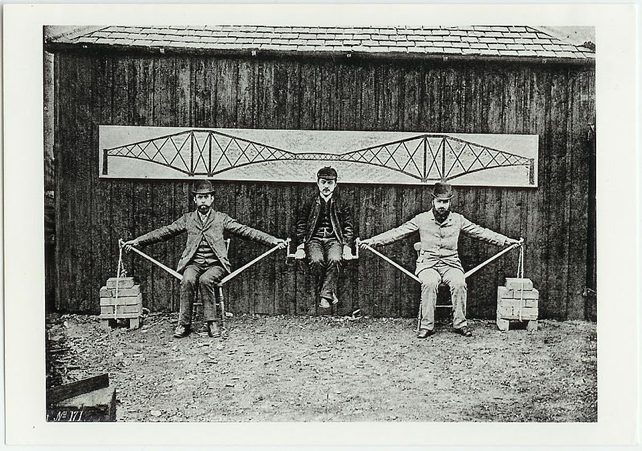
\includegraphics[width=0.6\textwidth]{images/suspension-bridge-principle}
\end{center}

The design was a cantilever bridge: the lower members (steel beams) are under compression; the upper members in tension.

\end{frame}



\begin{frame}
\frametitle{Quebec Bridge is Falling Down...}

The principle of cantilever bridges is sound; they're used all over the world.\\
\quad Including as the replacement for the bridge that failed!

What might be some other causes of failure?

\end{frame}



\begin{frame}
\frametitle{Manufacturing of the Steel}

As only half the bridge was built, it was possible to inspect the steel support beams still in fabrication.

\vspace{5em}

\begin{quote}
The work done by the Phoenix Bridge Company in making the detail drawings and in planning and carrying out the erection and by the Phoenix Iron Company in fabricating the material was good, and the steel used was of good quality.  
\end{quote}

So it isn't that. But, are engineers responsible for checking these things?

\end{frame}



\begin{frame}
\frametitle{Penny-Wise, Pound-Foolish}

There was insufficient money to perform anything more than the absolute minimum number tests required.


Engineering is not about getting the job done at the cheapest possible rate -- it's about reasonable pay for competent engineering work.


A practitioner shall uphold the principle of adequate compensation for engineering work.

\end{frame}



\begin{frame}
\frametitle{The Designer}

Cooper had designed bridges across North America before...

Cooper, however, was almost 70 years old at the time of the disaster and had only visited the construction site twice.

An engineer can have his or her licence revoked, suspended or limited in cases where the practitioner is found incompetent.

\end{frame}



\begin{frame}
\frametitle{Don't Ignore the Warnings}

There were bent members for almost a month prior to the collapse and workers were skipping work rather than work on a bridge they felt was dangerous.


Listen to your contractors and workers:  you might have an engineering degree, but they will, at least for a few decades, more experience than you.

Do not be embarrassed if you make a mistake -- contractors know engineers are human, too, and they appreciate it when they acknowledge their mistakes...

\end{frame}



\begin{frame}
\frametitle{This isn't supposed to bend...}

The engineers all argued as to the cause of the bent members even though the inspectors stated that they were true (straight) when installed.

Theories:
\begin{itemize}
 \item They were bent while they were being built in Phoenix.
 \item They were damaged while being unloaded from the trains.
 \item They were damaged while being installed.
\end{itemize}

None of which were correct...

Norman McLure was the only engineer who recognized the danger.

Engineers must co-operate in working with other professionals engaged on a project and act towards them with courtesy and good faith.

\end{frame}



\begin{frame}
\frametitle{So Pretty}

Cooper had curved members added to the structure for aesthetic reasons.

These increased the secondary stresses and added difficulties to fabrication.

\begin{center}
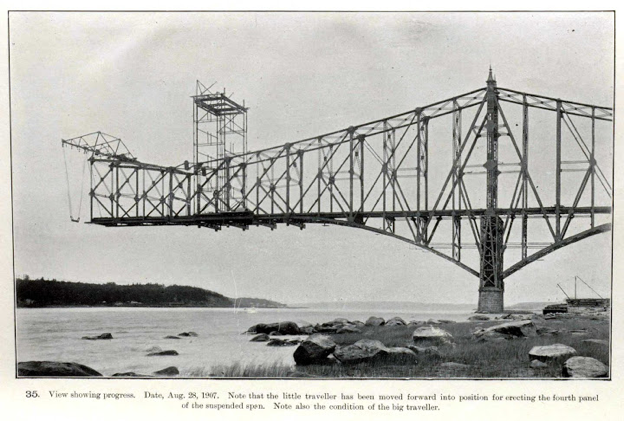
\includegraphics[width=0.6\textwidth]{images/curved-beams}
\end{center}

The most important thing must always be public safety, not how ``pretty'' it is.

\end{frame}



\begin{frame}
\frametitle{Final Plans}

No set of final designs was ever prepared -- all work was based on designs that had modifications and calculations using different notations.

This can lead to tremendous confusion and disarray.

Any final designs, plans, drawings, or any other document must be sealed, dated and signed by the engineer.


Contractors and officials are taught that a drawing should only be relied upon if it has been correctly sealed.

\end{frame}



\begin{frame}
\frametitle{Competence}

The failure on the part of the Quebec Bridge and Railway Company to appoint an experienced bridge engineer to the position of chief engineer was a mistake.


Hoare restarted work after Norman McLure stopped construction two days prior to the collapse.


Hoare seemed to be more interested in maintaining the schedule.


An engineer should not undertake work the practitioner is not competent to perform by virtue of the practitioner's training and experience.

\end{frame}



\begin{frame}
\frametitle{Check Yourself...}

The bridge was designed by Szlapka, the chief designer for Phoenix.

Cooper approved this design without thoroughly checking the calculations.


It is wrong to seal any final drawing, specification, plan, report or other document not actually prepared or checked by the practitioner!


\end{frame}



\begin{frame}
\frametitle{Egos}

Cooper refused to submit his designs to an engineer who would have been appointed by the Ministry of Railways and Canals.

Cooper claimed this would undermine his authority.

Engineers must understand it does not undermine their authority to have someone else validate their work.
\end{frame}



\begin{frame}
\frametitle{The Aftermath}

\begin{center}
 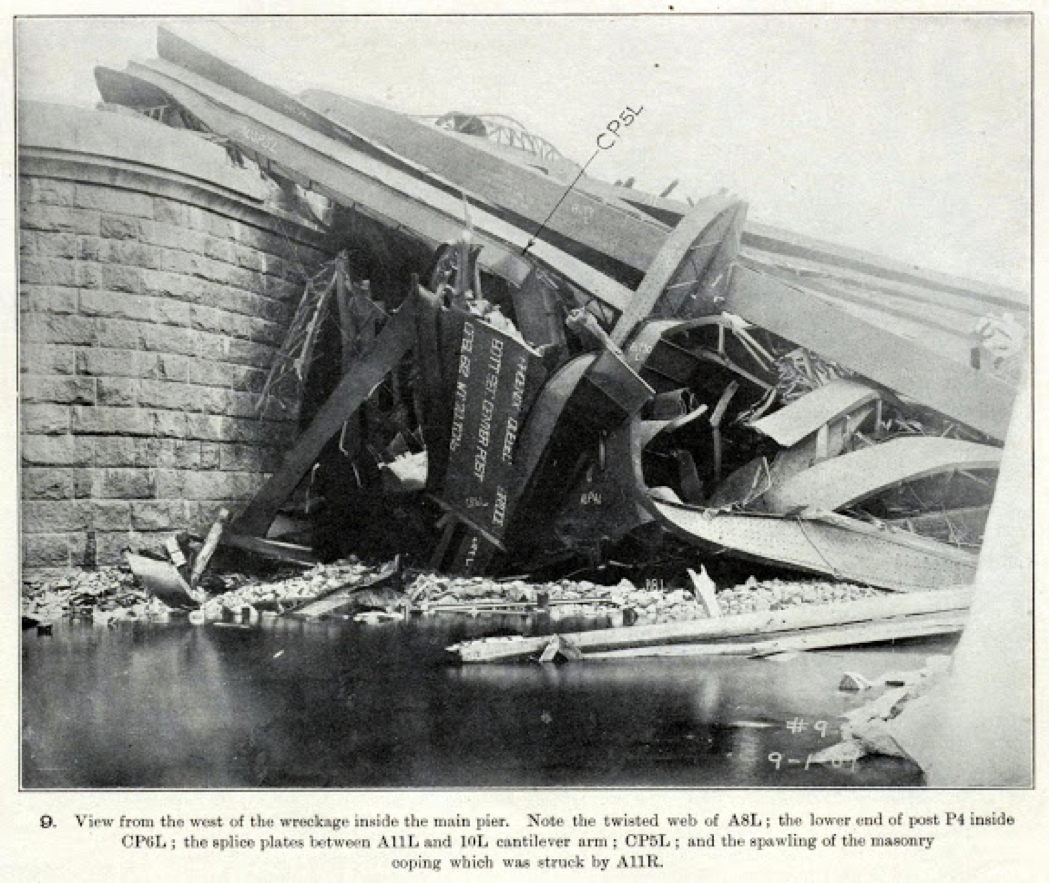
\includegraphics[width=0.8\textwidth]{images/collapse1}
\end{center}


\end{frame}
\begin{frame}
\frametitle{The Aftermath}

\begin{center}
 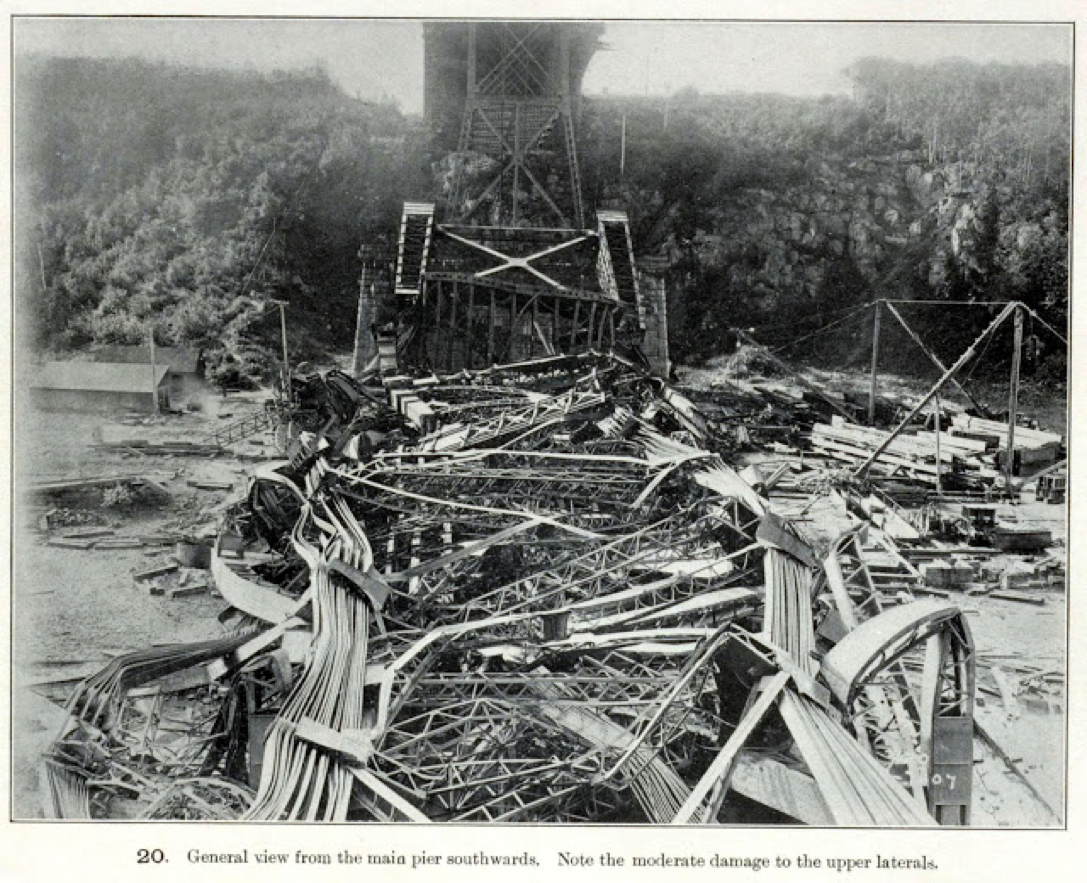
\includegraphics[width=0.8\textwidth]{images/collapse2}
\end{center}


\end{frame}

\begin{frame}
\frametitle{The Aftermath}

\begin{center}
 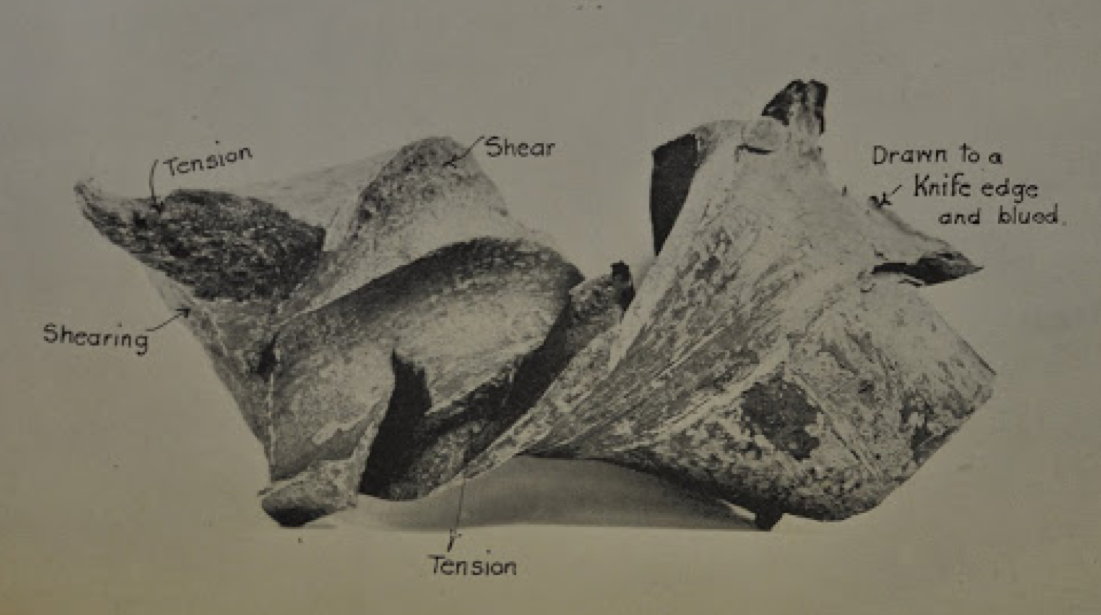
\includegraphics[width=0.8\textwidth]{images/collapse3}
\end{center}


\end{frame}

\begin{frame}
\frametitle{The Aftermath}

\begin{center}
 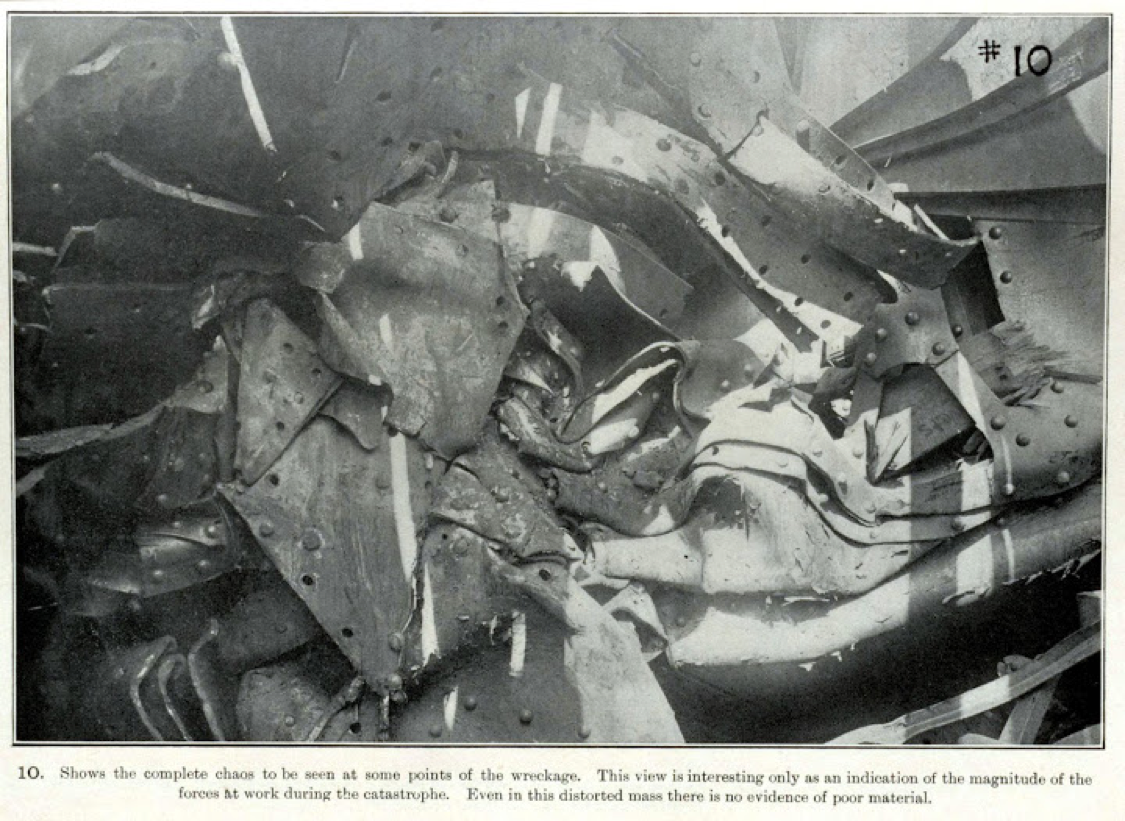
\includegraphics[width=0.8\textwidth]{images/collapse4}
\end{center}


\end{frame}

\begin{frame}
\frametitle{The Aftermath}

\begin{center}
 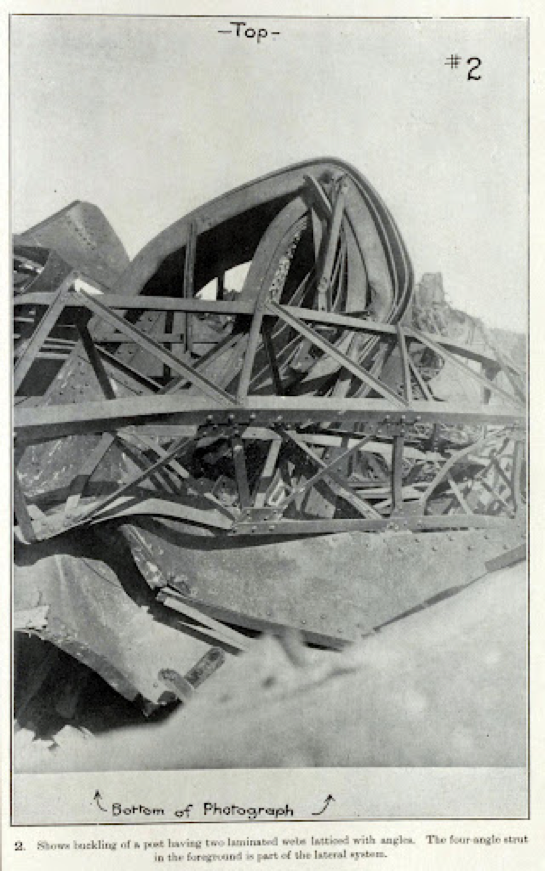
\includegraphics[width=0.4\textwidth]{images/collapse5}
 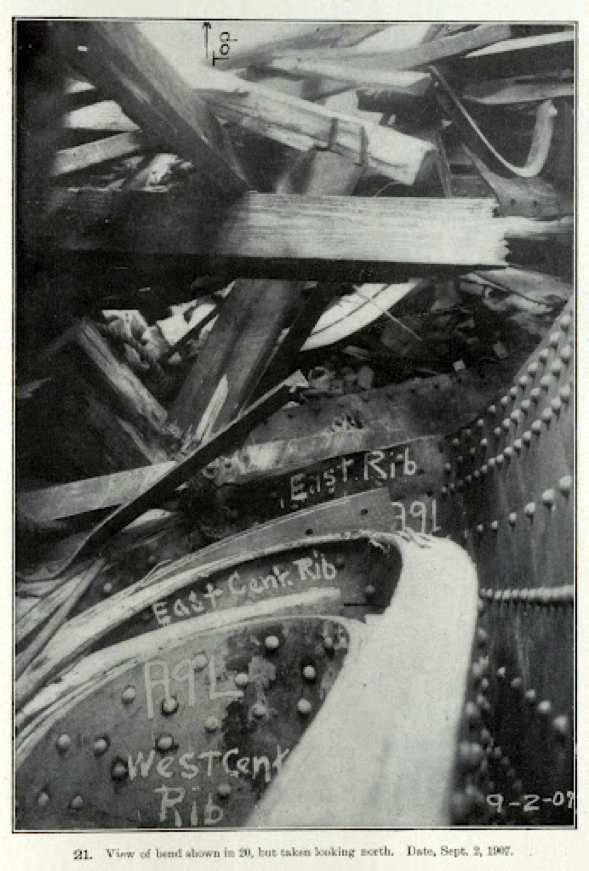
\includegraphics[width=0.4\textwidth]{images/collapse6}
\end{center}

\end{frame}



\begin{frame}
\frametitle{Incompetence}

The Discipline Committee may find a member of the Association or a holder of a temporary licence, a provisional licence or a limited licence to be incompetent if in its opinion,

\begin{enumerate}[(a)]
\item the member or holder has displayed in his or her professional responsibilities a lack of knowledge, skill or judgment or disregard for the welfare of the public of a nature or to an extent that demonstrates the member or holder is unfit to carry out the responsibilities of a professional engineer; or
\item the member or holder is suffering from a physical or mental condition or disorder of a nature and extent making it desirable in the interests of the public or the member or holder that the member or holder no longer be permitted to engage in the practice of professional engineering or that his or her practice of professional engineering be restricted. 
\end{enumerate}

\end{frame}




\begin{frame}
\frametitle{Professional Misconduct}

As a consequence of a number of engineering disasters, behaviour detrimental to acceptable practice has been collectively labeled \alert{professional misconduct}.

Section 72 (2) of O.Reg. 941 gives the definition of professional misconduct.

You do not have to memorize these; they will be provided for you in any exam.
\end{frame}



\begin{frame}
\frametitle{Professional Misconduct}

72. (2) For the purposes of the Act and this Regulation, ``professional misconduct'' means:


(a) negligence; that is, an act or an omission in the carrying out of  the work of a practitioner that constitutes a failure to maintain  the standards that a reasonable and prudent practitioner would  maintain in the circumstances


\end{frame}


\begin{frame}
\frametitle{Professional Misconduct}

72. (2) For the purposes of the Act and this Regulation, ``professional misconduct'' means:

(b) failure to make reasonable provision for the safeguarding of  life, health or property of a person who may be affected by the  work for which the practitioner is responsible

\end{frame}


\begin{frame}
\frametitle{Professional Misconduct}

72. (2) For the purposes of the Act and this Regulation, ``professional misconduct'' means:

(c) failure to act to correct or report a situation that the practitioner  believes may endanger the safety or the welfare of the public

\end{frame}

\begin{frame}
\frametitle{Professional Misconduct}

72. (2) For the purposes of the Act and this Regulation, ``professional misconduct'' means:

(d) failure to make responsible provision for complying with  applicable statutes, regulations, standards, codes, by-laws and  rules in connection with work being undertaken by or under the  responsibility of the practitioner

\end{frame}

\begin{frame}
\frametitle{Professional Misconduct}

72. (2) For the purposes of the Act and this Regulation, ``professional misconduct'' means:

(e) signing or sealing a final drawing, specification, plan, report or  other document not actually prepared or checked by the  practitioner

\end{frame}


\begin{frame}
\frametitle{Professional Misconduct}

72. (2) For the purposes of the Act and this Regulation, ``professional misconduct'' means:

(f)  failure of a practitioner to present clearly to the practitioner's  employer the consequences to be expected from a deviation  proposed in work, if the professional engineering judgment of  the practitioner is overruled by non-technical authority in cases  where the practitioner is responsible for the technical adequacy  of professional engineering work

\end{frame}

\begin{frame}
\frametitle{Professional Misconduct}

72. (2) For the purposes of the Act and this Regulation, ``professional misconduct'' means:

(g) breach of the Act or regulations, other than an action that is  solely a breach of the code of ethics

\end{frame}

\begin{frame}
\frametitle{Professional Misconduct}

72. (2) For the purposes of the Act and this Regulation, ``professional misconduct'' means:

(h) undertaking work the practitioner is not competent to perform  by virtue of the practitioner's training and experience

\end{frame}

\begin{frame}
\frametitle{Professional Misconduct}

72. (2) For the purposes of the Act and this Regulation, ``professional misconduct'' means:

(i)  failure to make prompt, voluntary and complete disclosure of  an interest, direct or indirect, that might in any way be, or be  construed as, prejudicial to the professional judgment of the  practitioner in rendering service to the public, to an employer or  to a client...

\end{frame}


\begin{frame}
\frametitle{Professional Misconduct}

72. (2) For the purposes of the Act and this Regulation, ``professional misconduct'' means:

(i)  ... and in particular, without limiting the generality of the  foregoing, carrying out any of the following acts without making  such a prior disclosure:

\begin{enumerate}
\item Accepting compensation in any form for a particular service from more than one party.
\item Submitting a tender or acting as a contractor in respect of work upon which the practitioner may be performing as a professional engineer.
\item Participating in the supply of material or equipment to be used by the employer or client of the practitioner.
\item Contracting in the practitioner's own right to perform professional engineering services for other than the practitioner's employer.
\item Expressing opinions or making statements concerning matters within the practice of professional engineering of public interest where the opinions or statements are inspired or paid for by other interests,
\end{enumerate}


\end{frame}



\begin{frame}
\frametitle{Secret Commissions}

Note that any secret commissions are also considered criminal under the Criminal Code of Canada:

\textbf{Secret commissions}\\
426. (1) Every one commits an offence who\\
(a) directly or indirectly, corruptly gives, offers or agrees to give or offer to an agent or to anyone for the benefit of the agent  --  or, being an agent, directly or indirectly, corruptly demands, accepts or offers or agrees to accept from any person, for themselves or another person  --  any reward, advantage or benefit of any kind as consideration for doing or not doing, or for having done or not done, any act relating to the affairs or business of the agent's principal, or for showing or not showing favour or disfavour to any person with relation to the affairs or business of the agent's principal; or


\end{frame}



\begin{frame}
\frametitle{Secret Commissions}

(b) with intent to deceive a principal, gives to an agent of that principal, or, being an agent, uses with intent to deceive his principal, a receipt, an account or other writing
\begin{enumerate}[i)]
\item in which the principal has an interest,
\item that contains any statement that is false or erroneous or defective in any material particular, and
\item that is intended to mislead the principal.
\end{enumerate}

\textbf{Privity to offence}\\
(2) Every one commits an offence who is knowingly privy to the commission of an offence under subsection (1).

\textbf{Punishment}\\
(3) A person who commits an offence under this section is guilty of an indictable offence and liable to imprisonment for a term not exceeding five years.


\end{frame}



\begin{frame}
\frametitle{Indictable Offence}

What is an indictable offence?
\begin{itemize}
\item It requires either an indictment following a preliminary hearing to determine if there is a \textit{prima facie} case
\item Allows for a trial by jury
\item Can apply for a pardon after ten years
\item Also known as a felony
\end{itemize}


This contrasts with summary conviction offences:
\begin{itemize}
	\item Maximum sentence is 6 months or a fine of \$5,000
	\item Must be charged within six months and no fingerprints required
	\item Can apply for a pardon after five years
	\item Also known as a misdemeanour
\end{itemize}


\end{frame}


\begin{frame}
\frametitle{Professional Misconduct}

72. (2) For the purposes of the Act and this Regulation, ``professional misconduct'' means:

(j) conduct or an act relevant to the practice of professional 	engineering that, having regard to all the circumstances, would 	reasonably be regarded by the engineering profession as 	disgraceful, dishonourable or unprofessional

\end{frame}


\begin{frame}
\frametitle{Professional Misconduct}

72. (2) For the purposes of the Act and this Regulation, ``professional misconduct'' means:

(k) failure by a practitioner to abide by the terms, conditions or 	limitations of the practitioner's licence, provisional licence, 	limited licence, temporary licence or certificate

\end{frame}


\begin{frame}
\frametitle{Professional Misconduct}

72. (2) For the purposes of the Act and this Regulation, ``professional misconduct'' means:

(l)  failure to supply documents or information requested by an 	investigator acting under section 33 of the Act

\end{frame}


\begin{frame}
\frametitle{Professional Misconduct}

72. (2) For the purposes of the Act and this Regulation, ``professional misconduct'' means:

(m) permitting, counselling or assisting a person who is not a 	practitioner to engage in the practice of professional 	engineering except as provided for in the Act or the regulations

\end{frame}


\begin{frame}
\frametitle{Professional Misconduct}

72. (2) For the purposes of the Act and this Regulation, ``professional misconduct'' means:

(n) harassment; that is, engaging in a course of vexatious 	comment or conduct that is known or ought reasonably to be 	known as unwelcome and that might reasonably be regarded 	as interfering in a professional engineering relationship

\end{frame}



\begin{frame}
\frametitle{How to Avoid Professional Misconduct}
\begin{enumerate}[(a)]

	\item Don't be negligent.
	\item Try to preserve life, health, property.
	\item Correct/report dangerous situations.
	\item Comply with statutes, regulations, codes. by-laws...
	\item Check anything you sign/seal/date.
	\item If a non-technical authority requires a dangerous deviation from
a design, you must point this out clearly and preferably in writing.
	\item Abide by the PEA and O.Reg.941
	\item Only engage in work in which you are competent
	\item Disclose any potential conflicts of interest
	\item Don't behave disgracefully, dishonourably, or unprofessionally.
	\item Obey the terms/conditions/limitations of the license. 
	\item Cooperate with any investigation.
	\item Don't encourage/support unlicensed people practicing
	\item Don't harass people.
\end{enumerate}

\end{frame}


\begin{frame}
\frametitle{References \& Disclaimer}
\bibliographystyle{alphaurl}
\setbeamertemplate{bibliography item}{\insertbiblabel}
{\scriptsize
\bibliography{290}
}
\vfill

{\tiny Disclaimer: the material presented in these lectures slides is intended for use in the course ECE~290 at the University of Waterloo and should not be relied upon as legal advice. Any reliance on these course slides by any party for any other purpose are the responsibility of such parties.  The author(s) accept(s) no responsibility for damages, if any, suffered by any party as a result of decisions made or actions based on these course slides for any other purpose than that for which it was intended.\par}


\end{frame}


\end{document}

